\documentclass{article}

\usepackage[letterpaper,left=1.5cm,right=1.5cm]{geometry}
\usepackage[utf8]{inputenc}
\usepackage[spanish]{babel}
\usepackage{graphicx}
\usepackage{pdfpages}
\usepackage{subfigure}
\usepackage{float}
\usepackage{fancyhdr}
\usepackage{appendix}
\usepackage{hyperref}

\hypersetup{
    colorlinks=true,
    linkcolor=black,
    filecolor=magenta,      
    urlcolor=blue,
}

\pagestyle{fancy}

\usepackage{times}

\usepackage{color}
\definecolor{gray97}{gray}{.97}
\definecolor{gray75}{gray}{.75}
\definecolor{gray45}{gray}{.45}

\usepackage{listings}
\lstset{ frame=Ltb,
framerule=0pt,
aboveskip=0.5cm,
framextopmargin=3pt,
framexbottommargin=3pt,
framexleftmargin=0.4cm,
framesep=0pt,
rulesep=.4pt,
backgroundcolor=\color{gray97},
rulesepcolor=\color{black},
%
stringstyle=\ttfamily,
showstringspaces = false,
basicstyle=\small\ttfamily,
commentstyle=\color{gray45},
keywordstyle=\bfseries,
%
numbers=left,
numbersep=15pt,
numberstyle=\tiny,
numberfirstline = false,
breaklines=true,
}

% minimizar fragmentado de listados
\lstnewenvironment{listing}[1][]
{\lstset{#1}\pagebreak[0]}{\pagebreak[0]}

\lstdefinestyle{consola}
{basicstyle=\scriptsize\bf\ttfamily,
backgroundcolor=\color{gray75},
}

\lstdefinestyle{C}
{language=C,
}




\begin{document}
\begin{titlepage}
  \begin{center}
    \Huge{Universidad Nacional Autónoma de México}

    \Huge{Facultad de Ingeniería}
    \vfill

    
\includegraphics[scale=.3]{../img/UNAM_INGENIERIA}
    \vfill
    \Large{Primera Entrega Compilador}

    
    \vfill
    \LARGE{\textbf{Wombat}}
    \vfill
  \end{center}  

  \Large{Datos del Cliente:
    
    \hspace{2cm}} Ing.\ Norberto Jesus Ortigoza Marquez
  \vfill
  
  \Large{Equipo de Desarrollo:
    
    \hspace{2cm}Romero Andrade Cristian\hfill -\hfill PMP, Arquitecto
    
    \hspace{2cm}Arguelles Macosay Mariana\hfill -\hfill Integradora, Tester}
  \vfill
  \Large{Entrega V 0.1: 16 de septiembre del 2019}
  

  % \vfill
  % \Large{Alumno: Romero Andrade Cristian}
  
  
\end{titlepage}

\tableofcontents{}

\section{Introducción}

\begin{flushright}
\textit{Un compilador para un pequeño Subconjunto de C,}  
\end{flushright}


Este proyecto trata acerca de crear un compilador en uno de los lenguajes de
programación permitidos, en este caso hemos elegido Elixir como el lenguaje
del proyecto. Para poder empezar debemos saber ¿Qué es un compilador?, un
compilador es de forma sencilla un programa que traduce un lenguaje a lenguaje
máquina es decir un lenguaje de alto nivel (palabras entendibles que puedan
expresar que queremos que haga un programa) a lenguaje maquina (conjunto
de números cuyo significado es directamente una orden al microprocesador).
Para la creación de un compilador existen ciertos procesos o pasos para poder
hacer las traducciones o compilaciones dependiendo sea el caso y la estructura
que tendrá el compilador, debido a la complejidad de los compiladores, en esta
o primera entrega solo haremos una parte de un compilador, aun así manteniendo
una estructura completa.

\section{Plan de Proyecto}

\subsection{Descripción del Proyecto}

El proyecto total consiste en un compilador de escala altamente reducida de
\textit{C} la cual consiste en lo siguiente:

\begin{lstlisting}[style=C]
int main() {
  return (3+4 <+ 4 || 1&& != 3>-6);

}
\end{lstlisting}

Para esta primera entrega el alcance llega a compilar el siguiente código

\begin{lstlisting}[style=C]
int main() {
  return 2;
}
\end{lstlisting}


\begin{figure}[H]
  \centering
  \subfigure{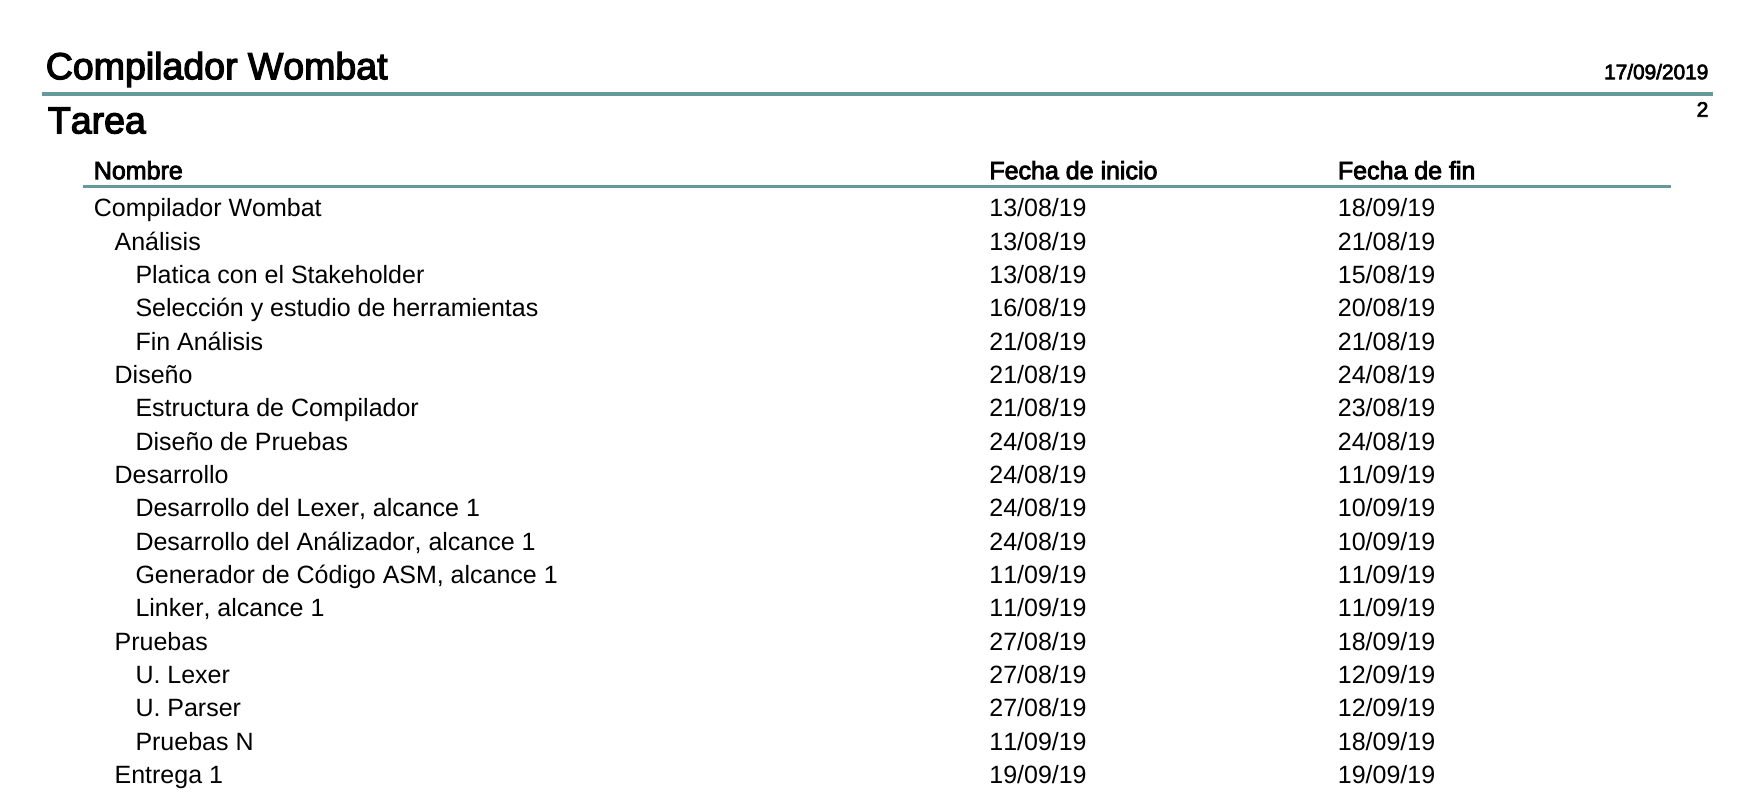
\includegraphics[width=17cm]{../img/pag-2}}
\end{figure}
\begin{figure}[H]
  \subfigure{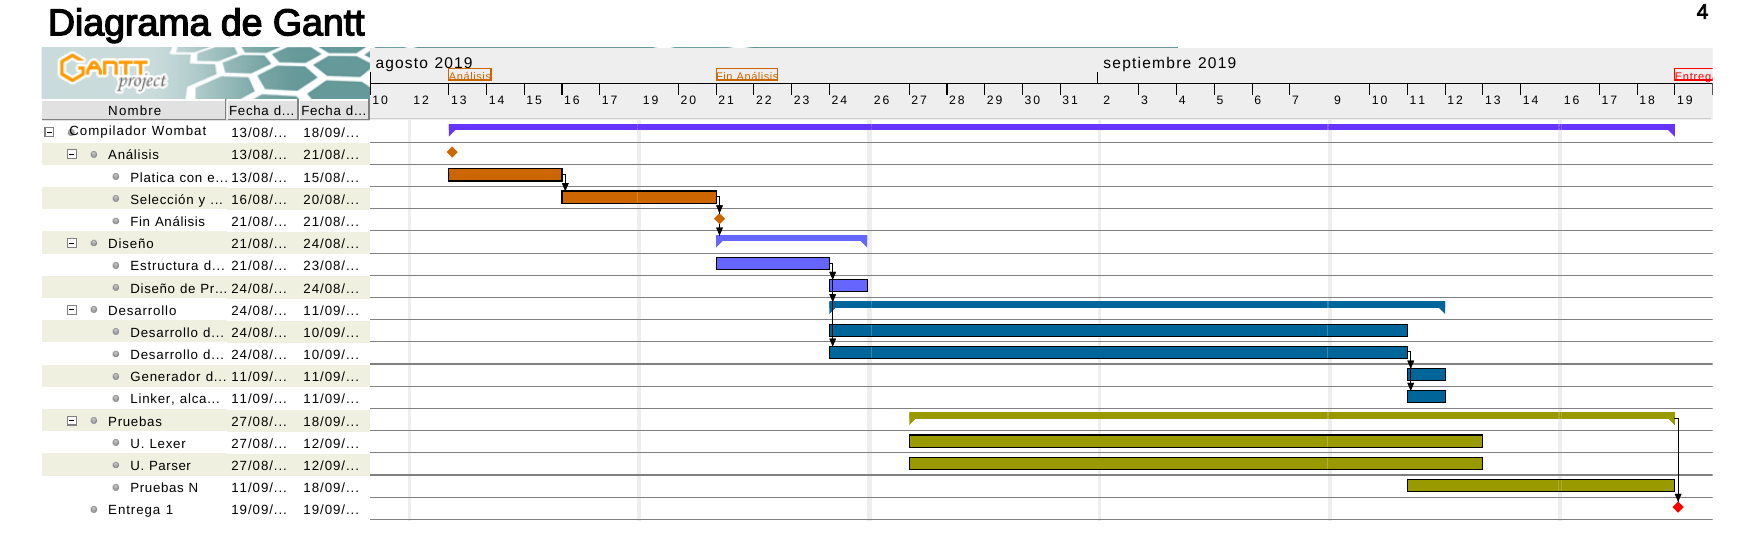
\includegraphics[width=17cm]{../img/pag-4}}
\end{figure}

Las próximas tareas al cerrar esta entrega, a parte de la adición de los
operadores unarios, será obtener el error de compilación junto con el número
de línea.



\subsection{Entorno de Trabajo}
\begin{itemize}
\item  Por petición del cliente todo entrégale relacionado con
  el proyecto se llevará a través de la plataforma de \href{https://github.com}
  {GitHub}.
  Más adelante se describe como se esta organizado el proyecto.
\item Se utilizará Elixir por las facilidades del lenguaje para el desarrollo
  específico del proyecto.
\item El editor es libre para cada desarrollador, aunque se recomienda el uso
  de \textit{Visual Studio Code} y \textit{Emacs} por el soporte del lenguaje
  (vscode-elixir y alchemist-mode respectivamente).
  
\item Se usará \textit{gcc} para enlazar el código ensamblador con la máquina.
\item Por ende se utiliza el gestor de versiones git.

\end{itemize}

\subsection{Actividades del equipo}

Se espera la siguiente rutina para el desarrollo del proyecto:

\begin{itemize}
\item Se trabajará en la rama \textit{dev}, cada fusión con \textit{master} se
  aprobará siempre y cuando la adición de un funcionamiento este completa y
  no haya cambios con el objetivo del proyecto.
\item Toda comunicación va a ser a través de \textit{Discord} y otro medio de
  mensajería instantánea.
\end{itemize}

\section{Arquitectura del Compilador}

\begin{figure}[H]
  \centering
  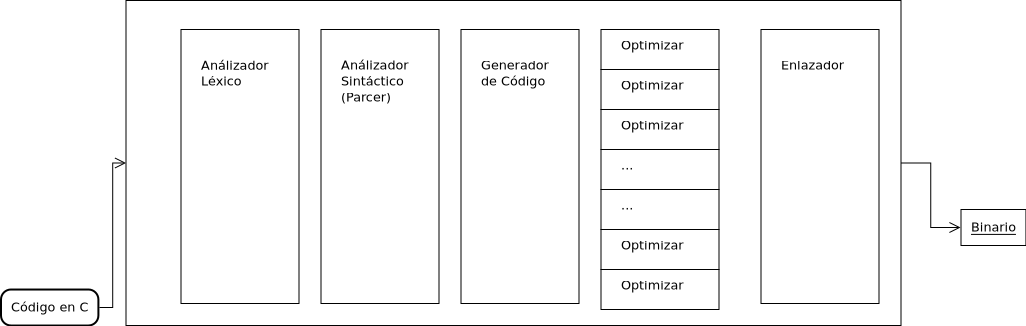
\includegraphics[width=17cm]{../img/Compilador}
\end{figure}

La arquitectura del compilador es simple utilizado el gestor de proyectos de \textit{elixir}
\textit{mix}, la cual genera las herramientas suficientes para las pruebas y compilación. La estructura que se decidió fue la siguiente:

\begin{itemize}
\item \_build
\item config
\item ejemplo
  \begin{itemize}
  \item return\_2.c
  \end{itemize}
\item lib
  \begin{itemize}
  \item compiladorwombat.ex
  \item wc2
    \begin{itemize}
    \item analizador.ex
    \item arbol.ex
    \item code\_gen.tex
    \item lexer.ex
    \item linker.ex
    \end{itemize}
  \item Makefile
  \item miscelanea
  \item mix.exs
  \item mix.lock
  \item README.md
  \item test
    \begin{itemize}
    \item compilador\_wombat\_test.exs
    \item stage\_1\footnote{Pruebas de Nora}
    \item test\_helper.exs
    \end{itemize}

  \end{itemize}

\end{itemize}

Ya que así se tiene separado las etapas del compilador y es fácil extender y dar mantenimiento a dicha
estructura tomando a todos los archivos necesarios de manera independiente.

\section{Plan de Pruebas y de ``Suites''}

El plan consiste en pasado un tiempo de desarrollo de los módulos del
compilador, se comenzará las pruebas mediante una  simple regla, ``Lo
que se debe de recibir, lo que se debe de mandar'', por ejemplo en el
caso del lexer, lo que este recibe es una lista de cadenas de caracteres
[``int'', ``main'', etc] y lo que debe de mandar en una lista y/o tupla de
\textit{tokens} [\textbf{:kint}, \textbf{:kmain}, etc]. Ya completado esta ``etapa''
de pruebas, se comenzará con las pruebas de \textbf{Nora}, la cual se espera solo
tener errores en sentencias especificas conservando el funcionamiento original.

\section{Conclusiones}

Gracias a la clase de compiladores nos fue posible definir una buena estructura
para el programa, por ahora el programa funciona, aunque solo acepta lo básico
y ciertas palabras clave, por lo que todavía no se puede considerar un compilador
completo ni usar como uno. Se aprendió que existen diversas herramientas que
facilitan la creación de compiladores. Para esta primera entrega podemos decir
que se ha realizado con éxito.


\appendix
\addappheadtotoc
\appendixpage
Repositorio del Proyecto \hfill$<$\url{https://github.com/hiphoox/c201-wombat}$>$



\end{document}
